\documentclass{beamer}
\usetheme{Montpellier}

\usepackage{color}
\usepackage{amsfonts}
\usepackage{comment}

%%% Al parecer necesito esto en ubuntu para los acentos
%\usepackage[spanish]{babel}
%\selectlanguage{spanish}
%\usepackage[utf8]{inputenc}

\definecolor{myblue}{rgb}{0.25, 0, 0.75}
\definecolor{mygold}{rgb}{1,0.8,0.2}
\definecolor{gray}{rgb}{0.5, 0.5, 0.5}
\definecolor{lucia}{rgb}{0.8,0.4,0.7} 

\newcommand{\myurl}[1]{\href{http://#1}{\textcolor{gray}{\texttt{#1}}}}
\newcommand{\myem}[1]{\structure{#1}}
\newcommand{\myurlshort}[2]{\href{http://#1}{\textcolor{gray}{\textsf{#2}}}}

\newcommand{\RPackage}[1]{\textcolor{gray}{\textsf{#1}}}
\newcommand{\pl}[1]{\texttt{#1}}
\newcommand{\RCode}[1]{\texttt{#1}}
\newcommand{\RFunction}[1]{\textsf{#1}}
\newcommand{\RClass}[1]{\textcolor{mygold}{\textsf{#1}}}
\newcommand{\BIOCfunction}[1]{\textcolor{orange}{#1}}

\setbeamercolor{example text}{fg=lucia}
\setbeamertemplate{sections/subsections in toc}[ball unumbered]
\setbeamertemplate{frametitle continuation}[from second][]
\setbeamertemplate{itemize subitem}[triangle]
\setbeamertemplate{footline}[page number]
\setbeamertemplate{caption}[numbered]
\setbeamertemplate{navigation symbols}{}

\renewcommand{\footnotesize}{\fontsize{6.10}{12}\selectfont}

\def\argmax{\operatornamewithlimits{arg\,max}}
\def\argmin{\operatornamewithlimits{arg\,min}}

%%\bibliographystyle{plain}


\title{Seminar III: R/Bioconductor}
\author{Leonardo Collado Torres \\ lcollado@lcg.unam.mx \\  Bachelor in Genomic Sciences \\ \myurl{www.lcg.unam.mx/\string~lcollado/}}
\date{
August - December, 2009
}








\usepackage{Sweave}
\begin{document}

\begin{frame}[allowframebreaks]
  \titlepage
\end{frame}

\section*{Class outline}

\begin{frame}[allowframebreaks]
  \frametitle{Genomic Plots}
  \tableofcontents[hideallsubsections]
\end{frame}

%%%%%%%%%%%%%%%%%%%%%%%%%%%%%%%%%%%%%%%%%%%%%%%%%%%%%%%%%%%%%%%%%%%%%%%%%%%
\section{Intro}

\begin{frame}[allowframebreaks]
  \frametitle{About}
  \begin{itemize}
  \item On this short class we'll learn how to make some plots that are focused on \emph{genomics}.
  \item The basic idea is a tool that enables you to visualize \emph{tracks} of information.
  \end{itemize}
\end{frame}

\begin{frame}[allowframebreaks, fragile]
  \frametitle{Session packages}
  \begin{itemize}
  \item Install commands:
\begin{Schunk}
\begin{Sinput}
> install.packages("RMySQL")
> source("http://bioconductor.org/biocLite.R")
> biocLite("rtracklayer")
> biocLite("humanStemCell")
> biocLite("GenomeGraphs")
\end{Sinput}
\end{Schunk}
  \end{itemize}
\end{frame}

%%%%%%%%%%%%%%%%%%%%%%%%%%%%%%%%%%%%%%%%%%%%%%%%%%%%%%%%%%%%%%%%%%%%%%%%%%%
\section{GenomeGraphs}

\begin{frame}[allowframebreaks]
  \frametitle{GenomeGraphs}
  \begin{itemize}
  \item It uses \pl{grid} graphics\footnote{Just like lattice.} and works great with \BIOCfunction{biomaRt}.
  \item The syntax is different and \BIOCfunction{longer} from what we are used to.
  \item Much more flexible than other packages, and I find it to be more stable :)
  \item Who are the authors of the package?
  \item For more \alert{info}, check this \myurlshort{www.ncbi.nlm.nih.gov/pubmed/19123956}{paper}.
  \end{itemize}
\end{frame}

\begin{frame}[allowframebreaks, fragile]
  \frametitle{gdPlot}
  \begin{itemize}
  \item To start off, we'll use the \BIOCfunction{gdPlot} function, which is the main one.
\begin{Schunk}
\begin{Sinput}
> library(GenomeGraphs)
\end{Sinput}
\end{Schunk}
\begin{Schunk}
\begin{Sinput}
> `?`(gdPlot)
\end{Sinput}
\end{Schunk}
  \item What kind of object does it need as input?
  \item What determines the plotting order?
  \end{itemize}
\end{frame}

\begin{frame}[allowframebreaks]
  \frametitle{gdObjects}
  \begin{itemize}
  \item So we need to create a \pl{list} with \BIOCfunction{gdObjects}.
  \item How do we find them?
  \end{itemize}
\end{frame}

\begin{frame}[allowframebreaks, fragile]
  \frametitle{gdObjects II}
  \begin{itemize}
  \item You can always look at the examples from the \pl{gdPlot} help and find a few.
  \item I would either browse the package help using:
\begin{Schunk}
\begin{Sinput}
> help(package = GenomeGraphs)
\end{Sinput}
\end{Schunk}
  \item Or thanks to some previous info, I know that the functions that create this kind of objects start with \alert{make}. So we can use \BIOCfunction{apropos}.
\begin{Schunk}
\begin{Sinput}
> apropos("make")
\end{Sinput}
\end{Schunk}
  \end{itemize}
\end{frame}

\begin{frame}[allowframebreaks, fragile]
  \frametitle{makeBaseTrack}
  \begin{itemize}
  \item Lets create an object of class \pl{BaseTrack} using \BIOCfunction{makeBaseTrack}\footnote{Yes, it's a long name :P}. \scriptsize
\begin{Schunk}
\begin{Sinput}
> args(makeBaseTrack)
\end{Sinput}
\begin{Soutput}
function (base, value, strand, segmentation, dp = NULL) 
NULL
\end{Soutput}
\end{Schunk}
\normalsize
  \item The first arguments are quite simple.
  \begin{enumerate}
  \item \pl{base} has the position values; the $x$ coordinates.
  \item \pl{value} is the analog for the $y$ axis.
  \item \pl{strand} is just a "+" or "-" character.
  \end{enumerate}
  \item Lets create a simple track for positions 1 to 100 with random log-normal values.
\begin{Schunk}
\begin{Sinput}
> makeBaseTrack(1:100, rlnorm(100))
\end{Sinput}
\begin{Soutput}
Object of class 'BaseTrack':
 base position: 
[1] 1 2 3 4 5
Values: 
[1] 0.8592530 1.8658355 0.4555190
[4] 0.8784603 3.3690927

 There are 95 more rowscolor  =  orange 
lty  =  solid 
lwd  =  1 
size  =  5 
type  =  p 
\end{Soutput}
\end{Schunk}
  \end{itemize}
\end{frame}

\begin{frame}[allowframebreaks, fragile]
  \frametitle{makeBaseTrack II}
  \begin{itemize}
  \item The first lines print the \pl{head} for \pl{base} and \pl{value}. The next ones inform us of the graphical parameters such as \pl{lwd} (line width).
  \item Lets save our track into the object \pl{a} assigning it to the positive strand.
\begin{Schunk}
\begin{Sinput}
> a <- makeBaseTrack(1:100, rlnorm(100), 
+     strand = "+")
\end{Sinput}
\end{Schunk}
  \item Lets make the plot now :)
  \end{itemize}
\end{frame}

\begin{frame}[fragile, allowframebreaks]
  \frametitle{Simple gdPlot}
\begin{Schunk}
\begin{Sinput}
> gdPlot(a)
\end{Sinput}
\end{Schunk}
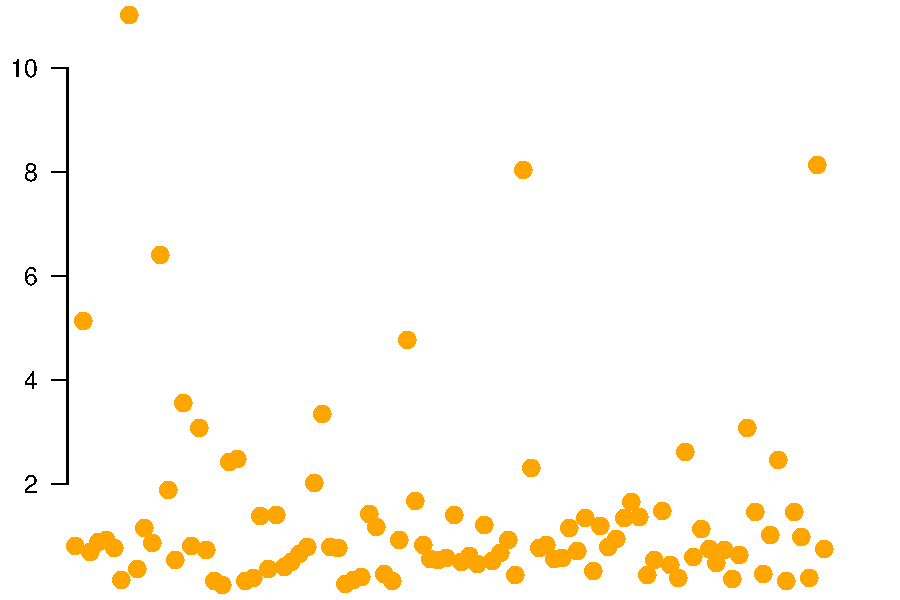
\includegraphics{plots/fig-010}
\end{frame}

\begin{frame}[allowframebreaks, fragile]
  \frametitle{gdPlot exercise}
  \begin{itemize}
  \item Now create and object \pl{b} using \BIOCfunction{makeBaseTrack} for the first 100 positions using random normal values and assign them to the negative strand.
  \item Then plot both \pl{a} and \pl{b} using \BIOCfunction{gdPlot}
  \end{itemize}
\end{frame}

\begin{frame}[fragile, allowframebreaks]
  \frametitle{Short solution}
\begin{Schunk}
\begin{Sinput}
> info <- list(makeBaseTrack(1:100, 
+     rlnorm(100), strand = "+"), 
+     makeBaseTrack(1:100, rnorm(100), 
+         strand = "-"))
> gdPlot(info)
\end{Sinput}
\end{Schunk}
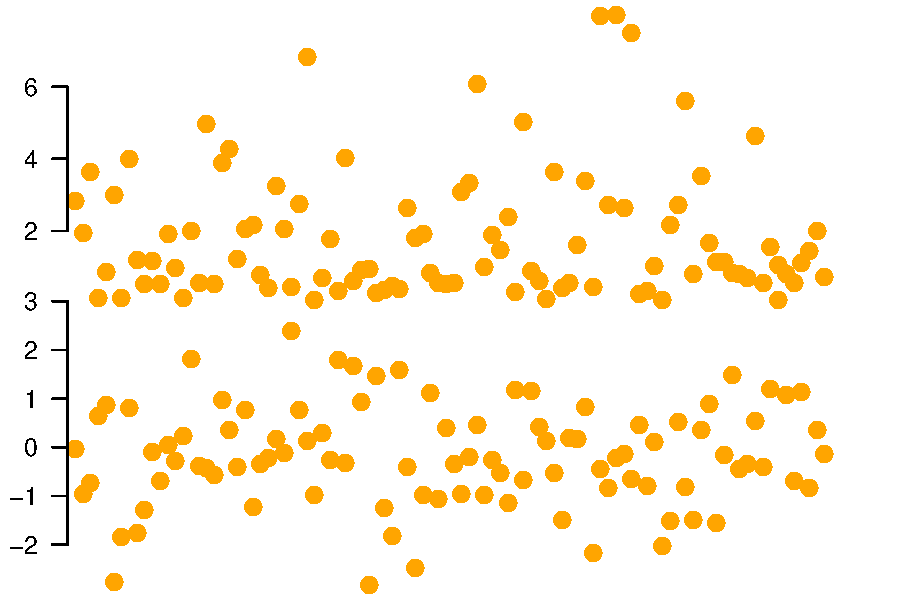
\includegraphics{plots/fig-011}
\end{frame}

\begin{frame}[fragile, allowframebreaks]
  \frametitle{What is the difference?}
\begin{Schunk}
\begin{Sinput}
> info2 <- list(makeBaseTrack(1:100, 
+     rlnorm(100), strand = "+"), 
+     makeBaseTrack(1:100, rnorm(100), 
+         strand = "-"), makeGenomeAxis())
> gdPlot(info2)
\end{Sinput}
\end{Schunk}
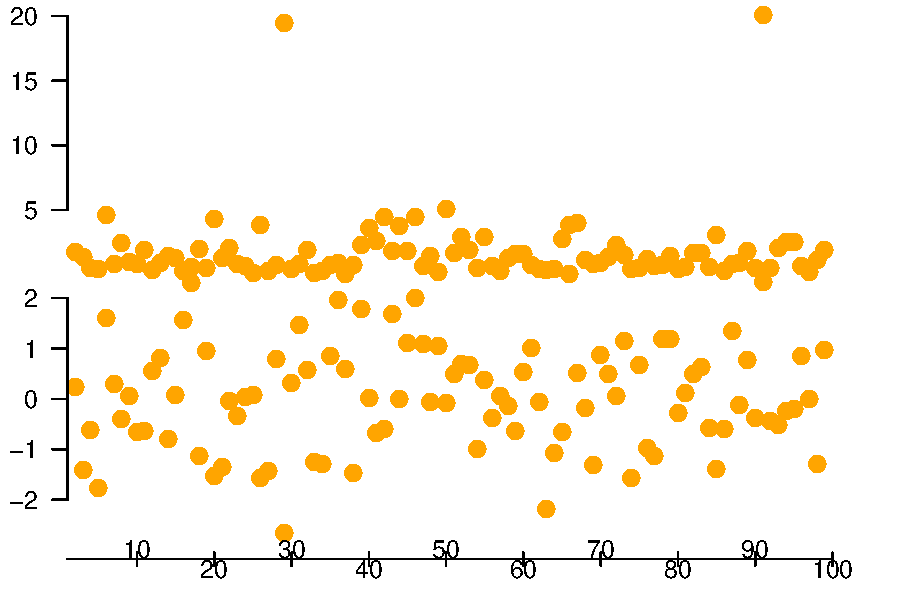
\includegraphics{plots/fig-012}
\end{frame}

\begin{frame}[allowframebreaks, fragile]
  \frametitle{DisplayPars}
  \begin{itemize}
  \item In \pl{GenomeGraphs}, to change graphical arguments we need to use the \BIOCfunction{DisplayPars} function.
  \item However, the arguments differ for every \pl{gdObject}. So we need to check them before using them.
  \item Lets go back to \pl{makeBaseTrack} and change the color of the negative strand values.
\begin{Schunk}
\begin{Sinput}
> b <- makeBaseTrack(1:100, rnorm(100), 
+     strand = "-", dp = DisplayPars(color = "blue"))
\end{Sinput}
\end{Schunk}
  \end{itemize}
\end{frame}

\begin{frame}[fragile, allowframebreaks]
  \frametitle{Changing colors}
\begin{Schunk}
\begin{Sinput}
> gdPlot(list(a, b, makeGenomeAxis()))
\end{Sinput}
\end{Schunk}
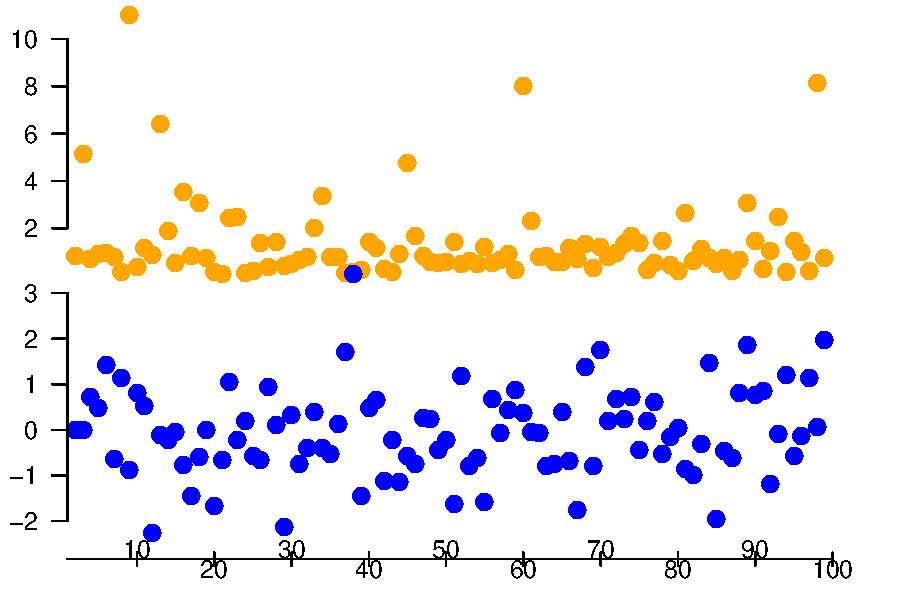
\includegraphics{plots/fig-014}
\end{frame}

\begin{frame}[allowframebreaks, fragile]
  \frametitle{Finding args}
  \begin{itemize}
  \item In practice, its better to find the arguments using \BIOCfunction{showDisplayOptions}
  \item For example:
\begin{Schunk}
\begin{Sinput}
> showDisplayOptions("BaseTrack")
\end{Sinput}
\begin{Soutput}
color  =  orange 
lty  =  solid 
lwd  =  1 
size  =  5 
type  =  p 
\end{Soutput}
\end{Schunk}
  \item How many graphical arguments does the genome axis object have?
  \end{itemize}
\end{frame}

\begin{frame}[allowframebreaks]
  \frametitle{Names}
  \begin{itemize}
  \item Say we want to add the strand names to our previous plots and to our axis.
  \item Any ideas? Remember that we are using a list.
  \end{itemize}
\end{frame}

\begin{frame}[fragile, allowframebreaks]
  \frametitle{gdPlot with names}
\begin{Schunk}
\begin{Sinput}
> gdPlot(list(`+` = a, `-` = b, Base = makeGenomeAxis()))
\end{Sinput}
\end{Schunk}
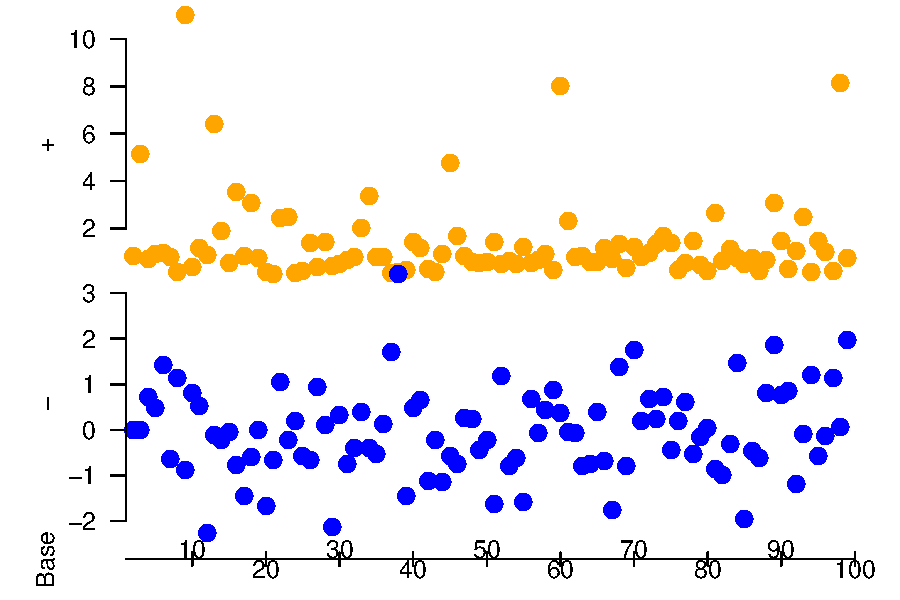
\includegraphics{plots/fig-016}
\end{frame}

\begin{frame}[allowframebreaks, fragile]
  \frametitle{Interaction with biomaRt}
  \begin{itemize}
  \item \pl{GenomeGraphs} can retrieve information from public databases using \pl{biomaRt}.
  \item To do so, we use the function \BIOCfunction{makeGeneRegion}: \scriptsize
\begin{Schunk}
\begin{Sinput}
> args(makeGeneRegion)
\end{Sinput}
\begin{Soutput}
function (start, end, chromosome, strand, biomart, dp = NULL) 
NULL
\end{Soutput}
\end{Schunk}
\normalsize
  \item The \pl{biomart} argument is a \pl{mart} object. Lets create one:
\begin{Schunk}
\begin{Sinput}
> bsub <- useMart("bacterial_mart_54", 
+     dataset = "bac_6_gene")
\end{Sinput}
\end{Schunk}
  \end{itemize}
\end{frame}

\begin{frame}[allowframebreaks]
  \frametitle{GeneRegion exercise}
  Using our \pl{bsub} mart,
  \begin{enumerate}
  \item Create a \pl{GeneRegion} object \pl{c} with info from the genes from the bases 12000 to 20000 for the positive strand.
  \item Create an object \pl{d} for those on the negative strand.
  \item Create a plot with the axis using \BIOCfunction{gdPlot}.
  \end{enumerate}
  You will need to get the chromosome name. You might want to use \pl{listAttributes} and/or do a simple \pl{getBM}, or check on web biomart, or guess it ;)
\end{frame}

\begin{frame}[allowframebreaks, fragile]
  \frametitle{Step by step solution}
  \begin{itemize}
  \item To find the chromsome name, I simply checked the attributes list. \scriptsize
\begin{Schunk}
\begin{Sinput}
> head(listAttributes(bsub))
\end{Sinput}
\begin{Soutput}
                   name
1       ensembl_gene_id
2 ensembl_transcript_id
3    ensembl_peptide_id
4           description
5       chromosome_name
6        start_position
            description
1       Ensembl Gene ID
2 Ensembl Transcript ID
3    Ensembl Protein ID
4           Description
5    Chromosome/plasmid
6       Gene Start (bp)
\end{Soutput}
\end{Schunk}
\normalsize
  \item Of course, we can verify this with by using \BIOCfunction{getBM}\footnote{I just modified one of the code lines we used on the \pl{biomaRt} class.}:
\begin{Schunk}
\begin{Sinput}
> res <- getBM(attributes = c("chromosome_name"), 
+     filters = c("start", "end"), 
+     values = list("1", "1000"), 
+     mart = bsub)
> res
\end{Sinput}
\begin{Soutput}
  chromosome_name
1      Chromosome
\end{Soutput}
\end{Schunk}
  \item Then we can get the info for the genes on the positive strand:
\begin{Schunk}
\begin{Sinput}
> c <- makeGeneRegion(12000, 20000, 
+     chromosome = "Chromosome", 
+     strand = "+", biomart = bsub)
\end{Sinput}
\end{Schunk}
  \item For the \pl{d} object, we use nearly the same code and we finish the job with \pl{gdPlot}:
\begin{Schunk}
\begin{Sinput}
> d <- makeGeneRegion(12000, 20000, 
+     chromosome = "Chromosome", 
+     strand = "-", biomart = bsub)
\end{Sinput}
\end{Schunk}
  \end{itemize}
\end{frame}

\begin{frame}[fragile, allowframebreaks]
  \frametitle{Resulting plot}
\begin{Schunk}
\begin{Sinput}
> gdPlot(list(`+` = c, `-` = d, Bsub = makeGenomeAxis()))
\end{Sinput}
\end{Schunk}
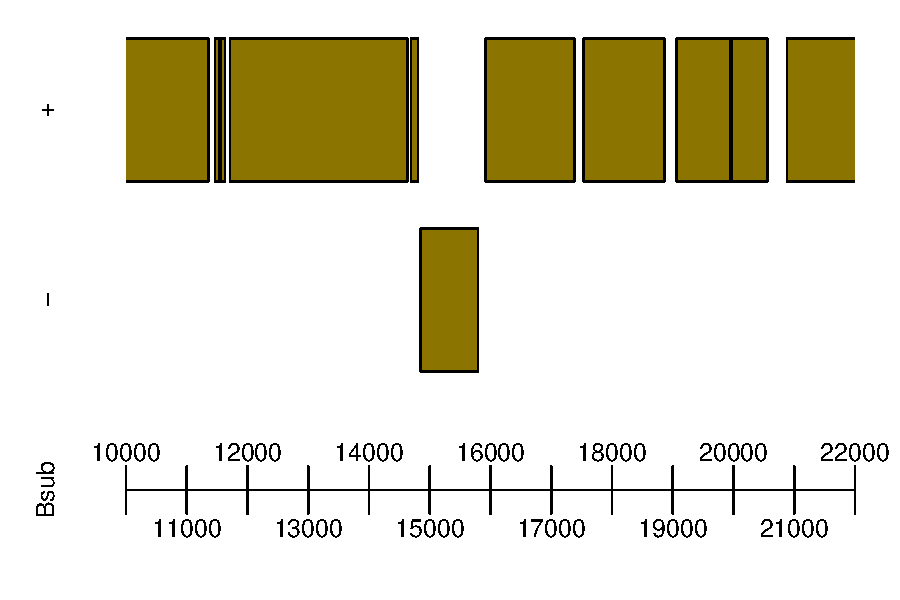
\includegraphics{plots/fig-023}
\end{frame}

\begin{frame}[allowframebreaks, fragile]
  \frametitle{Microarray data}
  \begin{itemize}
  \item Lets make more complicated plots with microarray data from David et al.
  \item We'll be using a different mart and the example dataset \alert{seqDataEx}
\begin{Schunk}
\begin{Sinput}
> mart <- useMart("ensembl", "scerevisiae_gene_ensembl")
> data("seqDataEx")
> head(seqDataEx$david)
\end{Sinput}
\begin{Soutput}
  chr location strand  expr
1   4  1300003     -1 -0.20
2   4  1300007      1  0.61
3   4  1300011     -1  0.07
4   4  1300015      1  1.25
5   4  1300019     -1 -0.29
6   4  1300023      1  0.61
\end{Soutput}
\end{Schunk}
  \item Lets take a peak at chromosome IV:
  \end{itemize}
\end{frame}

\begin{frame}[fragile, allowframebreaks]
  \frametitle{Basic plot}
\begin{Schunk}
\begin{Sinput}
> gdPlot(makeGeneRegion(10000, 50000, 
+     chr = "IV", strand = "+", biomart = mart), 
+     10000, 50000)
\end{Sinput}
\end{Schunk}
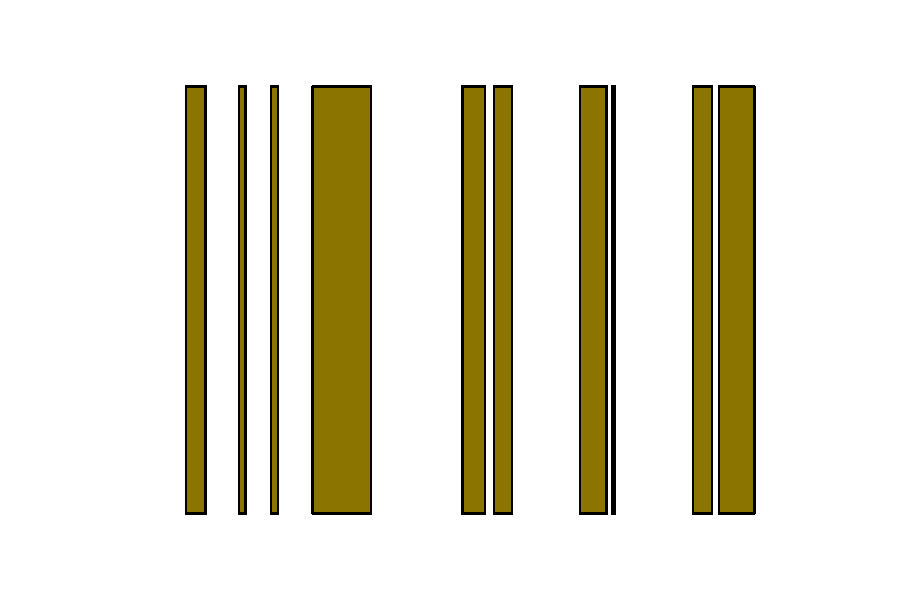
\includegraphics{plots/fig-025}
\end{frame}

\begin{frame}[allowframebreaks, fragile]
  \frametitle{Gene names}
  \begin{itemize}
  \item Lets add the \alert{gene names} (plot ids).
\begin{Schunk}
\begin{Sinput}
> showDisplayOptions("GeneRegion")
\end{Sinput}
\end{Schunk}
  \item What are the options to:
  \begin{enumerate}
  \item Add the gene names?
  \item Change the rotation angle of the names? 
  \item Change the letter size?
  \item Set the color? For example, to black.
  \end{enumerate}
  \item Re-make the previous plot with the names parallel to the $x$ axis, letter size 0.5 instead of 1, and in black.
  \end{itemize}
\end{frame}

\begin{frame}[fragile, allowframebreaks]
  \frametitle{Basic plot with names}
\begin{Schunk}
\begin{Sinput}
> gdPlot(makeGeneRegion(10000, 50000, 
+     chr = "IV", strand = "+", biomart = mart, 
+     dp = DisplayPars(plotId = TRUE, 
+         idRotation = 0, cex = 0.5, 
+         idColor = "black")), 10000, 
+     50000)
\end{Sinput}
\end{Schunk}
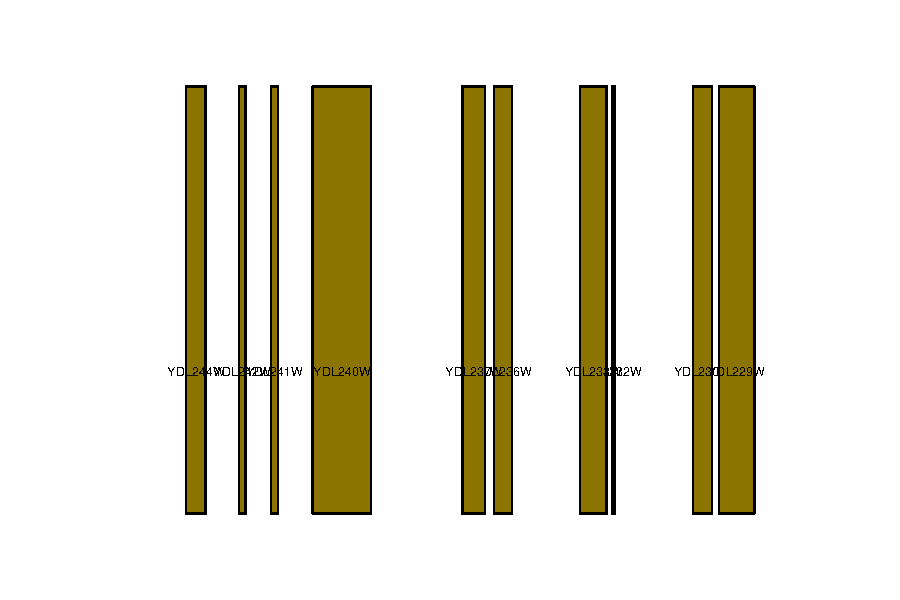
\includegraphics{plots/fig-027}
\end{frame}


\begin{frame}[allowframebreaks, fragile]
  \frametitle{GenericArray}
  \begin{itemize}
  \item Not much, right?
  \item Lets make one with the microarray data using \BIOCfunction{makeGenericArray}: \scriptsize
\begin{Schunk}
\begin{Sinput}
> args(makeGenericArray)
\end{Sinput}
\begin{Soutput}
function (intensity, probeStart, probeEnd, segmentation, dp = NULL) 
NULL
\end{Soutput}
\end{Schunk}
\normalsize
  \item For less typing, lets save the data into a shorter object:
\begin{Schunk}
\begin{Sinput}
> david <- seqDataEx$david
\end{Sinput}
\end{Schunk}
  \item We did a \pl{head} earlier on the data, so lets use \pl{location} for \pl{probeStart} and \pl{expr} for \pl{intensity} arguments respectively.
  \item As a short parenthesis, look at this neat trick:
\begin{Schunk}
\begin{Sinput}
> head(david[, "expr", drop = FALSE])
\end{Sinput}
\begin{Soutput}
   expr
1 -0.20
2  0.61
3  0.07
4  1.25
5 -0.29
6  0.61
\end{Soutput}
\begin{Sinput}
> head(david[, "expr", drop = TRUE])
\end{Sinput}
\begin{Soutput}
    1     2     3     4     5     6 
-0.20  0.61  0.07  1.25 -0.29  0.61 
\end{Soutput}
\end{Schunk}
  \item Neat eh? :) Lets use \BIOCfunction{makeGenericArray} now:
\begin{Schunk}
\begin{Sinput}
> e <- makeGenericArray(david[, "expr", 
+     drop = FALSE], david[, "location"])
\end{Sinput}
\end{Schunk}
  \end{itemize}
\end{frame}

\begin{frame}[fragile, allowframebreaks]
  \frametitle{GenericArray plot}
\begin{Schunk}
\begin{Sinput}
> gdPlot(list(e, makeGenomeAxis()))
\end{Sinput}
\end{Schunk}
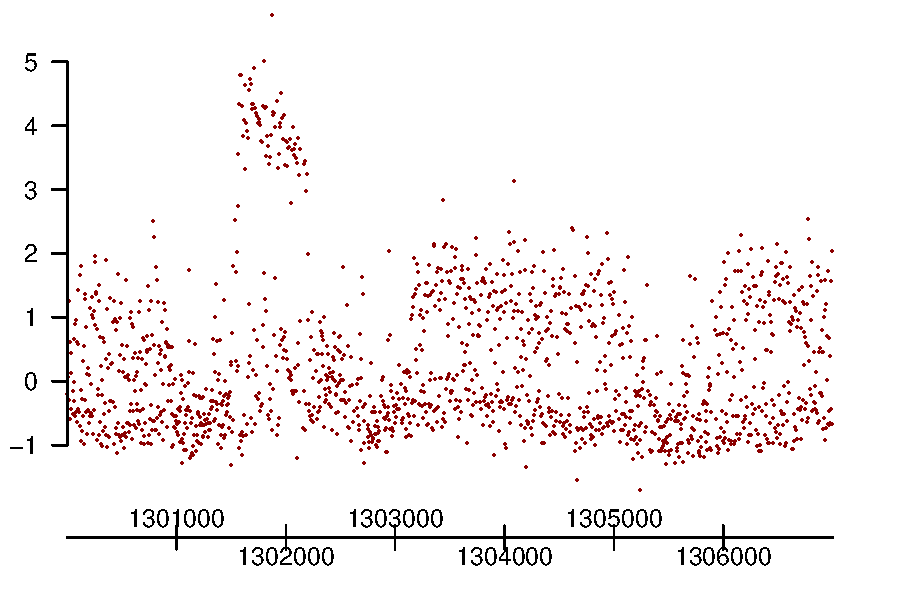
\includegraphics{plots/fig-032}
\end{frame}

\begin{frame}[allowframebreaks, fragile]
  \frametitle{Something... complicated :)}
  Now, lets make a \alert{complicated} plot
  \begin{itemize}
  \item One GeneRegion for each strand
  \item One GenericArray for each strand
    \end{itemize}
\end{frame}

\begin{frame}[allowframebreaks, fragile]
  \frametitle{Code:}
\begin{Schunk}
\begin{Sinput}
> df <- as.data.frame(seqDataEx$david)
> lst <- lapply(c("+", "-"), function(s) {
+     a <- as.matrix(subset(df, strand == 
+         ifelse(s == "+", 1, -1)))
+     c(makeGenericArray(a[, "expr", 
+         drop = FALSE], a[, "location"]), 
+         makeGeneRegion(start = min(df[, 
+             "location"]), end = max(df[, 
+             "location"]), chr = "IV", 
+             strand = s, biomart = mart, 
+             dp = DisplayPars(plotId = TRUE, 
+                 idRotation = 0, 
+                 cex = 0.5, idColor = "black")))
+ })
> yeastLst <- c(unlist(lst), makeGenomeAxis())
\end{Sinput}
\end{Schunk}
\end{frame}

\begin{frame}[fragile, allowframebreaks]
  \frametitle{A great plot!}
\begin{Schunk}
\begin{Sinput}
> gdPlot(yeastLst)
\end{Sinput}
\end{Schunk}
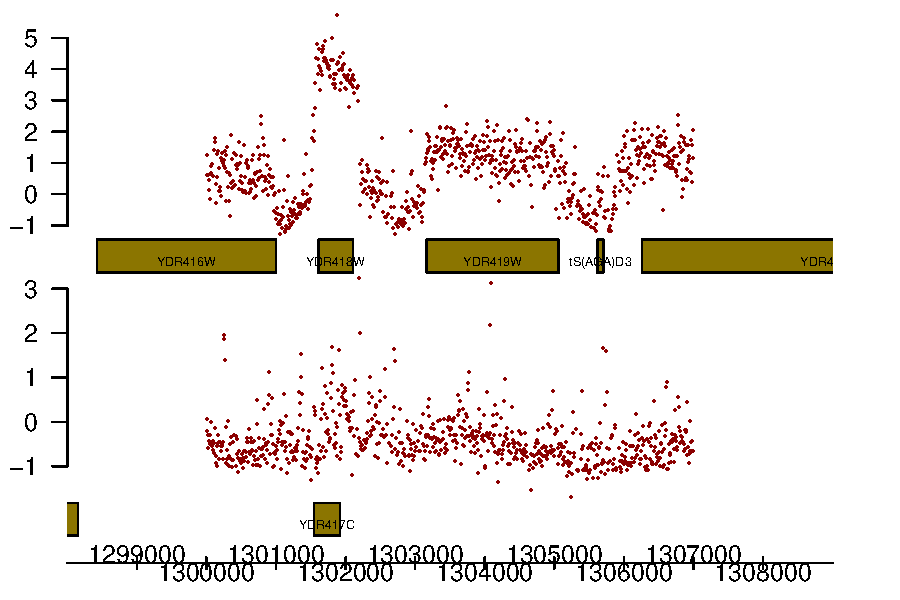
\includegraphics{plots/fig-034}
\end{frame}

\begin{frame}[allowframebreaks, fragile]
  \frametitle{Overlays}
  \begin{itemize}
  \item We can also add some rectangles and text to highlight interesting parts of the plot.
  \item To do so, we use \BIOCfunction{makeRectangleOverlay} and \BIOCfunction{makeTextOverlay}: \scriptsize
\begin{Schunk}
\begin{Sinput}
> args(makeRectangleOverlay)
\end{Sinput}
\begin{Soutput}
function (start, end, region = NULL, coords = c("genomic", "absolute"), 
    dp = NULL) 
NULL
\end{Soutput}
\begin{Sinput}
> args(makeTextOverlay)
\end{Sinput}
\begin{Soutput}
function (text, xpos, ypos, region = NULL, coords = c("genomic", 
    "absolute"), dp = NULL) 
NULL
\end{Soutput}
\end{Schunk}
\normalsize
  \end{itemize}
\end{frame}

\begin{frame}[allowframebreaks, fragile]
  \frametitle{Rectangle overlay exercise}
  \begin{itemize}
  \item Lets add a rectangle overlay to the previous plot.
  \item Which display argument enables us to make the rectangle semi-transparent? Use \BIOCfunction{showDisplayOptions}:
\begin{Schunk}
\begin{Sinput}
> showDisplayOptions("RectangleOverlay")
\end{Sinput}
\begin{Soutput}
alpha  =  0 
color  =  black 
fill  =  black 
lty  =  solid 
lwd  =  1 
\end{Soutput}
\end{Schunk}
  \item Add a rectangle overlay starting at 1301500, ending at 1302500, covering the first 2 panels and at exactly mid-transparency.
  \end{itemize}
\end{frame}

\begin{frame}[fragile, allowframebreaks]
  \frametitle{Solution :)}
\begin{Schunk}
\begin{Sinput}
> ovlay <- makeRectangleOverlay(1301500, 
+     1302500, region = c(1, 2), 
+     dp = DisplayPars(alpha = 0.5))
> gdPlot(yeastLst, overlays = c(ovlay))
\end{Sinput}
\end{Schunk}
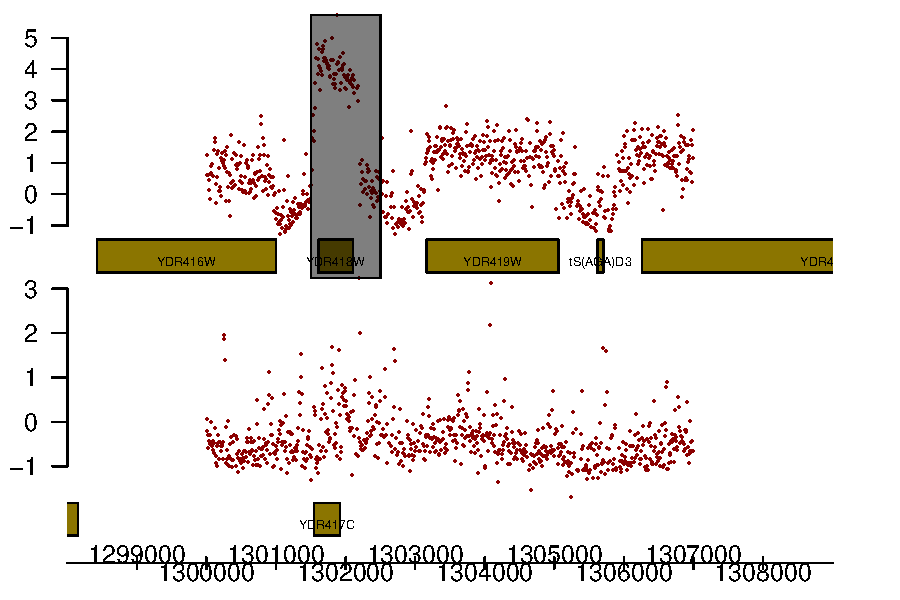
\includegraphics{plots/fig-037}
\end{frame}

\begin{frame}[allowframebreaks, fragile]
  \frametitle{With text}
  \begin{itemize}
  \item Now, lets add some text using \BIOCfunction{makeTextOverlay}
\begin{Schunk}
\begin{Sinput}
> tovlay <- makeTextOverlay("SpecialRegion", 
+     1303500, 0.75, region = c(1, 
+         1), dp = DisplayPars(color = "black"))
\end{Sinput}
\end{Schunk}
  \end{itemize}
\end{frame}

\begin{frame}[fragile, allowframebreaks]
  \frametitle{End result}
\begin{Schunk}
\begin{Sinput}
> gdPlot(yeastLst, overlays = c(ovlay, 
+     tovlay))
\end{Sinput}
\end{Schunk}
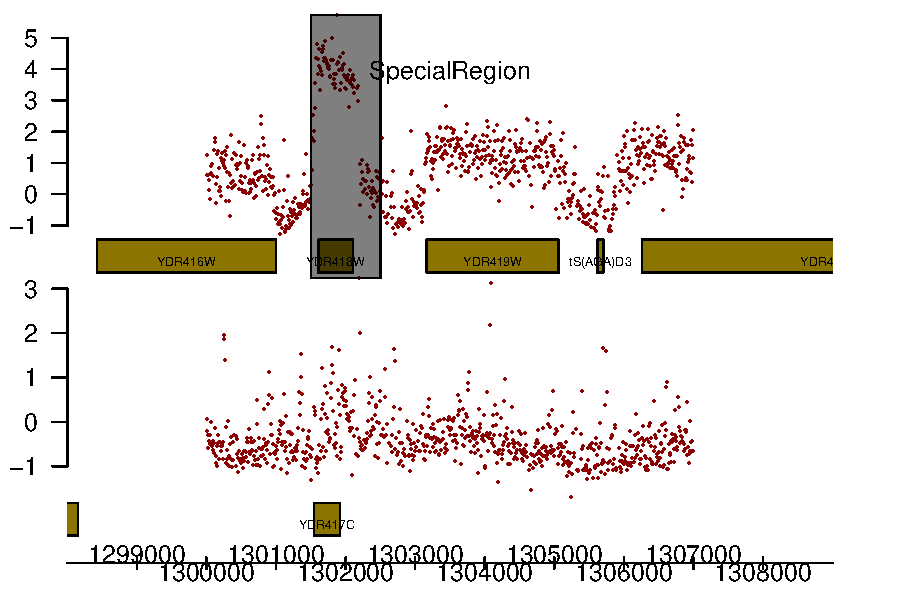
\includegraphics{plots/fig-039}
\end{frame}

\begin{frame}[allowframebreaks, fragile]
  \frametitle{Transcripts}
  \begin{itemize}
  \item For those of you who love splicing, \BIOCfunction{makeTranscript} will be most useful :)
  \item Lets take a look at gene ENSG00000168309: \scriptsize
\begin{Schunk}
\begin{Sinput}
> args(makeTranscript)
\end{Sinput}
\begin{Soutput}
function (id, type, biomart, dp = NULL) 
NULL
\end{Soutput}
\begin{Sinput}
> hMart <- useMart("ensembl", "hsapiens_gene_ensembl")
> trans <- makeTranscript("ENSG00000168309", 
+     biomart = hMart)
\end{Sinput}
\end{Schunk}
\normalsize
  \end{itemize}
\end{frame}

\begin{frame}[fragile, allowframebreaks]
  \frametitle{Alternative splicing}
\begin{Schunk}
\begin{Sinput}
> gdPlot(list(trans, makeGenomeAxis()))
\end{Sinput}
\end{Schunk}
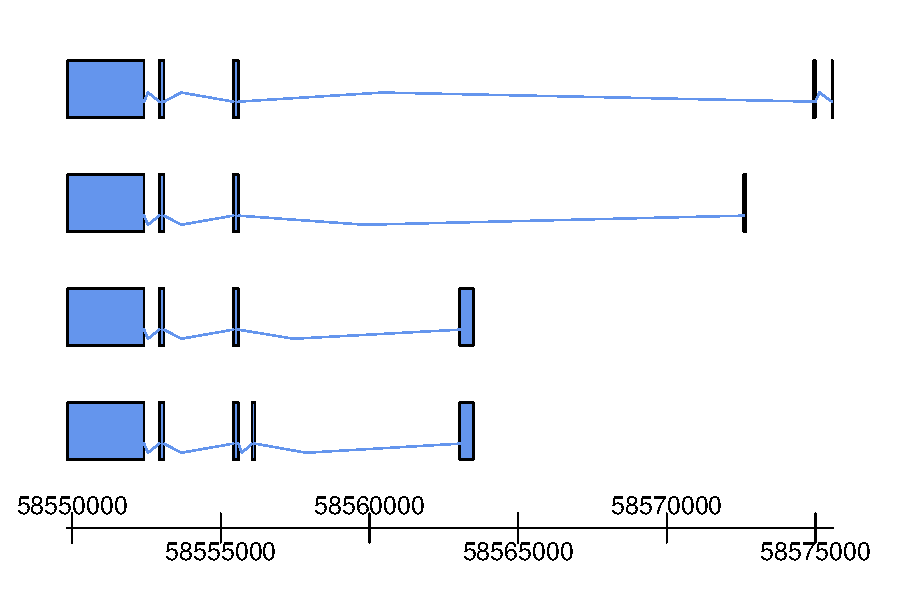
\includegraphics{plots/fig-041}
\end{frame}


\begin{frame}[allowframebreaks, fragile]
  \frametitle{Exons and gene models}
  \begin{itemize}
  \item Visualizing data can be troublesome when you have mixed ranges. Say a small exon, then a large intron, a medium exon, etc.
  \item If you have exon microarray data, then \BIOCfunction{makeExonArray} and \BIOCfunction{makeGeneModel} will be useful to you :)\footnote{For the curious ones, you can make custom annotation tracks using \BIOCfunction{makeAnnotationTrack}.} \scriptsize
\begin{Schunk}
\begin{Sinput}
> args(makeExonArray)
\end{Sinput}
\begin{Soutput}
function (intensity, probeStart, probeEnd, probeId, nProbes, 
    displayProbesets = FALSE, dp = NULL) 
NULL
\end{Soutput}
\begin{Sinput}
> args(makeGeneModel)
\end{Sinput}
\begin{Soutput}
function (start, end, chromosome, dp = NULL) 
NULL
\end{Soutput}
\end{Schunk}
\normalsize
  \item Here is an example using the \pl{unrData} dataset:
\begin{Schunk}
\begin{Sinput}
> data("unrData", package = "GenomeGraphs")
> class(unrData)
\end{Sinput}
\begin{Soutput}
[1] "matrix"
\end{Soutput}
\begin{Sinput}
> dim(unrData)
\end{Sinput}
\begin{Soutput}
[1] 117  33
\end{Soutput}
\begin{Sinput}
> head(unrPositions)
\end{Sinput}
\begin{Soutput}
  probesetId chromosome     start
1    2429278          1 115061081
2    2429279          1 115061152
3    2429280          1 115061275
4    2429281          1 115061486
5    2429282          1 115061888
6    2429283          1 115062185
       stop
1 115061119
2 115061198
3 115061409
4 115061528
5 115062089
6 115062218
\end{Soutput}
\end{Schunk}
  \item First we create the \BIOCfunction{exon track} which zooms into every exon, and then a \BIOCfunction{gene model} so we don't lose the forest :)
\begin{Schunk}
\begin{Sinput}
> exon <- makeExonArray(intensity = unrData, 
+     probeStart = unrPositions[, 
+         3], probeEnd = unrPositions[, 
+         4], probeId = as.character(unrPositions[, 
+         1]), nProbes = unrNProbes, 
+     dp = DisplayPars(color = "blue", 
+         mapColor = "dodgerblue2"), 
+     displayProbesets = FALSE)
> geneModel <- makeGeneModel(start = unrPositions[, 
+     3], end = unrPositions[, 4])
\end{Sinput}
\end{Schunk}
  \end{itemize}
\end{frame}

\begin{frame}[fragile, allowframebreaks]
  \frametitle{Example plot}
\begin{Schunk}
\begin{Sinput}
> gdPlot(list(exon, geneModel, makeGenomeAxis()))
\end{Sinput}
\end{Schunk}
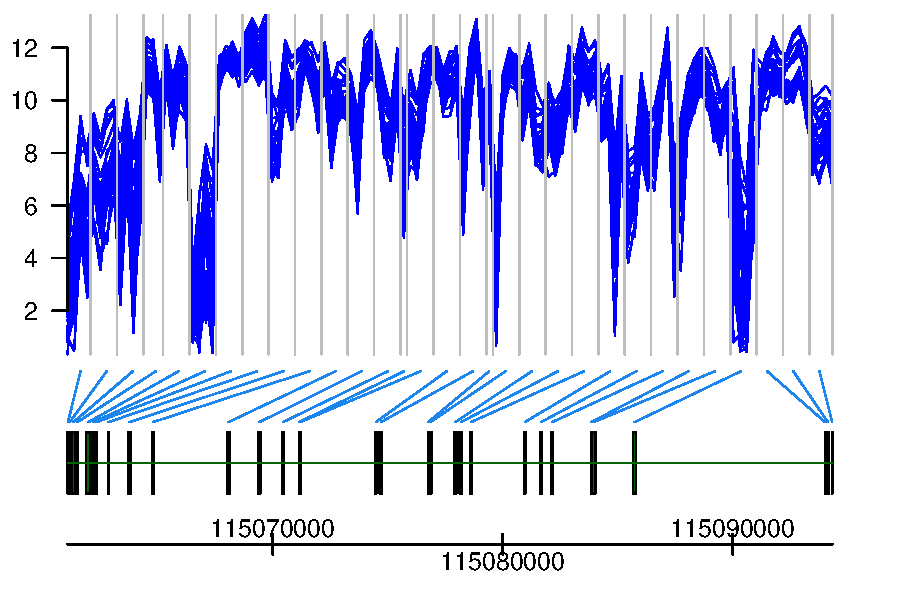
\includegraphics{plots/fig-045}
\end{frame}

\begin{frame}[allowframebreaks]
  \frametitle{Conclusions}
  \begin{itemize}
  \item Fast! Which is great for a quick exploration of your data by regions.
  \item Once you get the basics, its easy to use :)
  \item Very flexible!
  \item Has several handy functions for making genomic plots.
  \item Has the same limitations as other \pl{R} plots.
  \end{itemize}
\end{frame}

\begin{frame}[allowframebreaks]
  \frametitle{Credits}
  Nearly all the GenomeGraphs examples and exercises are from James Bullard's recent lab at BioC2009 available \myurlshort{www.bioconductor.org/workshops/2009/BioC2009/labs/biomaRtGenomeGraphs/GenomeGraphs.pdf}{here}. I modified some and expanded the explanations so it'd be easier to understand :)
\end{frame}

%%%%%%%%%%%%%%%%%%%%%%%%%%%%%%%%%%%%%%%%%%%%%%%%%%%%%%%%%%%%%%%%%%%%%%%%%%%
\section{rtracklayer}

\begin{frame}[allowframebreaks]
  \frametitle{Genome Browsers intro}
  \begin{itemize}
  \item I suppose that quite a few of you have heard about genome browsers, mainly the \BIOCfunction{UCSC Genome Browser}: \url{http://genome.ucsc.edu/}
  \item Its probably the most popular web tool for exploring genomes, specially eukaryotic genomes.
  \item Nowadays, they added quite a few nice tools and you can easily access data from a lot of information tracks: conservation, repeats, SNPs, etc.
  \item Other tools are BLAT (similar to BLAST), a PCR in silico tool, \ldots
  \end{itemize}
\end{frame}

\begin{frame}[allowframebreaks]
  \frametitle{GBs}
  \begin{itemize}
  \item Genome Browsers (GBs) are great for biologists. You don't need to write any code to use it.
  \item It simplifies the process of gathering data for you (aka, getting the tracks).
  \item You don't need any special software to use it, just a browser like Firefox.
  \item However, the formats are tedious to work with\ldots
  \item If you have custom tracks, you'll need to do lots of uploading.
  \end{itemize}
\end{frame}

\begin{frame}[allowframebreaks]
  \frametitle{rtracklayer}
  Michael Lawrence developed \BIOCfunction{rtracklayer} which lets you:
  \begin{enumerate}
  \item Import and export data to a GB (there are several formats).
  \item Create tracks using \BIOCfunction{IRanges}. And of course, manipulate them :)
  \item Browsing the data on the genome browser.
  \end{enumerate}
  \begin{itemize}
  \item However, I ran into problems when using the package recently :P
  \item Its not as easy to understand as \pl{GenomeGraphs}.
  \item So why learn about it? Michael is \alert{VERY} active on the mailing lists and I'm sure that he'll fix whatever is wrong right now. Also, GBs are very popular so you might need to use them in the future.
  \end{itemize}
\end{frame}

\begin{frame}[allowframebreaks]
  \frametitle{To learn}
  \begin{itemize}
  \item If you want to learn about the package, check the vignette and the \pl{R} code file available at \myurlshort{www.bioconductor.org/packages/devel/bioc/html/rtracklayer.html}{here}.
  \item Note that your computer might freeze on page 9 of the vignette file.
  \end{itemize}
\end{frame}

\begin{frame}[allowframebreaks, fragile]
  \frametitle{SessionInfo} \scriptsize
\begin{Schunk}
\begin{Sinput}
> sessionInfo()
\end{Sinput}
\begin{Soutput}
R version 2.10.0 Under development (unstable) (2009-07-25 r48998) 
i686-pc-linux-gnu 

locale:
 [1] LC_CTYPE=en_US.UTF-8      
 [2] LC_NUMERIC=C              
 [3] LC_TIME=en_US.UTF-8       
 [4] LC_COLLATE=en_US.UTF-8    
 [5] LC_MONETARY=C             
 [6] LC_MESSAGES=en_US.UTF-8   
 [7] LC_PAPER=en_US.UTF-8      
 [8] LC_NAME=C                 
 [9] LC_ADDRESS=C              
[10] LC_TELEPHONE=C            
[11] LC_MEASUREMENT=en_US.UTF-8
[12] LC_IDENTIFICATION=C       

attached base packages:
[1] grid      stats     graphics 
[4] grDevices utils     datasets 
[7] methods   base     

other attached packages:
[1] GenomeGraphs_1.5.1
[2] biomaRt_2.1.0     

loaded via a namespace (and not attached):
[1] RCurl_0.98-1 tools_2.10.0
[3] XML_2.6-0   
\end{Soutput}
\end{Schunk}
\end{frame}

\end{document}

